\section{Dynamic Modelling and Control of the Bicycle-Cargo System}

\subsection{Dynamic System Modelling} 

The studied system consists of a bicycle towing a cargo cart through a rigid mechanical linkage. This link is only used for steering guidance and does not contribute to the traction force. The main objective is to ensure that the rider perceives minimal additional effort, such that the overall behaviour remains similar to riding a standard bicycle. 

From a control perspective, the rider provides a reference motion in terms of speed and position, while the cargo cart is expected to follow this reference with minimal delay. The position error between the bicycle and the cargo cart is computed using a distance sensor, which provides feedback relative to an equilibrium state. 

The cargo cart is modelled as the plant of the system. Its rotational dynamics are described using the fundamental equation of rotational motion: 

\begin{equation*}
\sum \tau = J_{\Delta} \times \dot{\omega} 
\end{equation*} 
where $\tau$ is the total torque applied to the system, $J_{\Delta}$ is the equivalent moment of inertia, and $\omega$ is the angular velocity. 

The total torque is composed of the motor torque $\tau_m$ and a friction torque modelled as: 

\begin{equation*} 
\tau_f = -f \times \omega 
\end{equation*} 
where $f$ is the viscous friction coefficient. 

The resulting dynamic equation becomes: 

\begin{equation*} 
J_{\Delta} \dot{\omega} = \tau_m - f \omega 
\end{equation*} 

In the Laplace domain, this leads to: 
\begin{equation*} 
\omega(s) = \frac{\tau_m(s)}{J_{\Delta} s + f} 
\end{equation*} 

Since the linear velocity is related to angular velocity by the wheel radius $R$, we obtain: 

\begin{equation*} 
v(s) = R \times \omega(s) 
\end{equation*} 

Thus, the transfer function between motor torque and linear velocity is: 
\begin{equation*} 
\frac{v(s)}{\tau_m(s)} = \frac{R}{J_{\Delta} s + f} 
\end{equation*} 


\subsection{PI-Based Control Strategy} 
\label{subsec:Simulink_model}
Based on this model, a Simulink representation of the system was developed. The controlled system includes a feedback loop using a PI (Proportional-Integral) controller in order to regulate the position error between the bicycle and the cargo cart. 

Since the reference input is a ramp signal (representing the bicycle position over time), an integral action is required to ensure zero steady-state error and accurate tracking of the reference trajectory. 

The closed-loop Simulink model of the system is shown in Fig.~\ref{fig:simulink-closedloop}. 

The control error is defined as the difference between a desired relative position and the measured displacement between the bicycle and the cargo cart:
\begin{equation*}
    e(t) = e_{\text{ref}} - (x_{\text{bike}} - x_{\text{cart}})
\end{equation*}
where $e_{\text{ref}} = \SI{-0.5}{\meter}$ represents the desired equilibrium offset between both systems.

\begin{figure}[!h]

    \centering 
    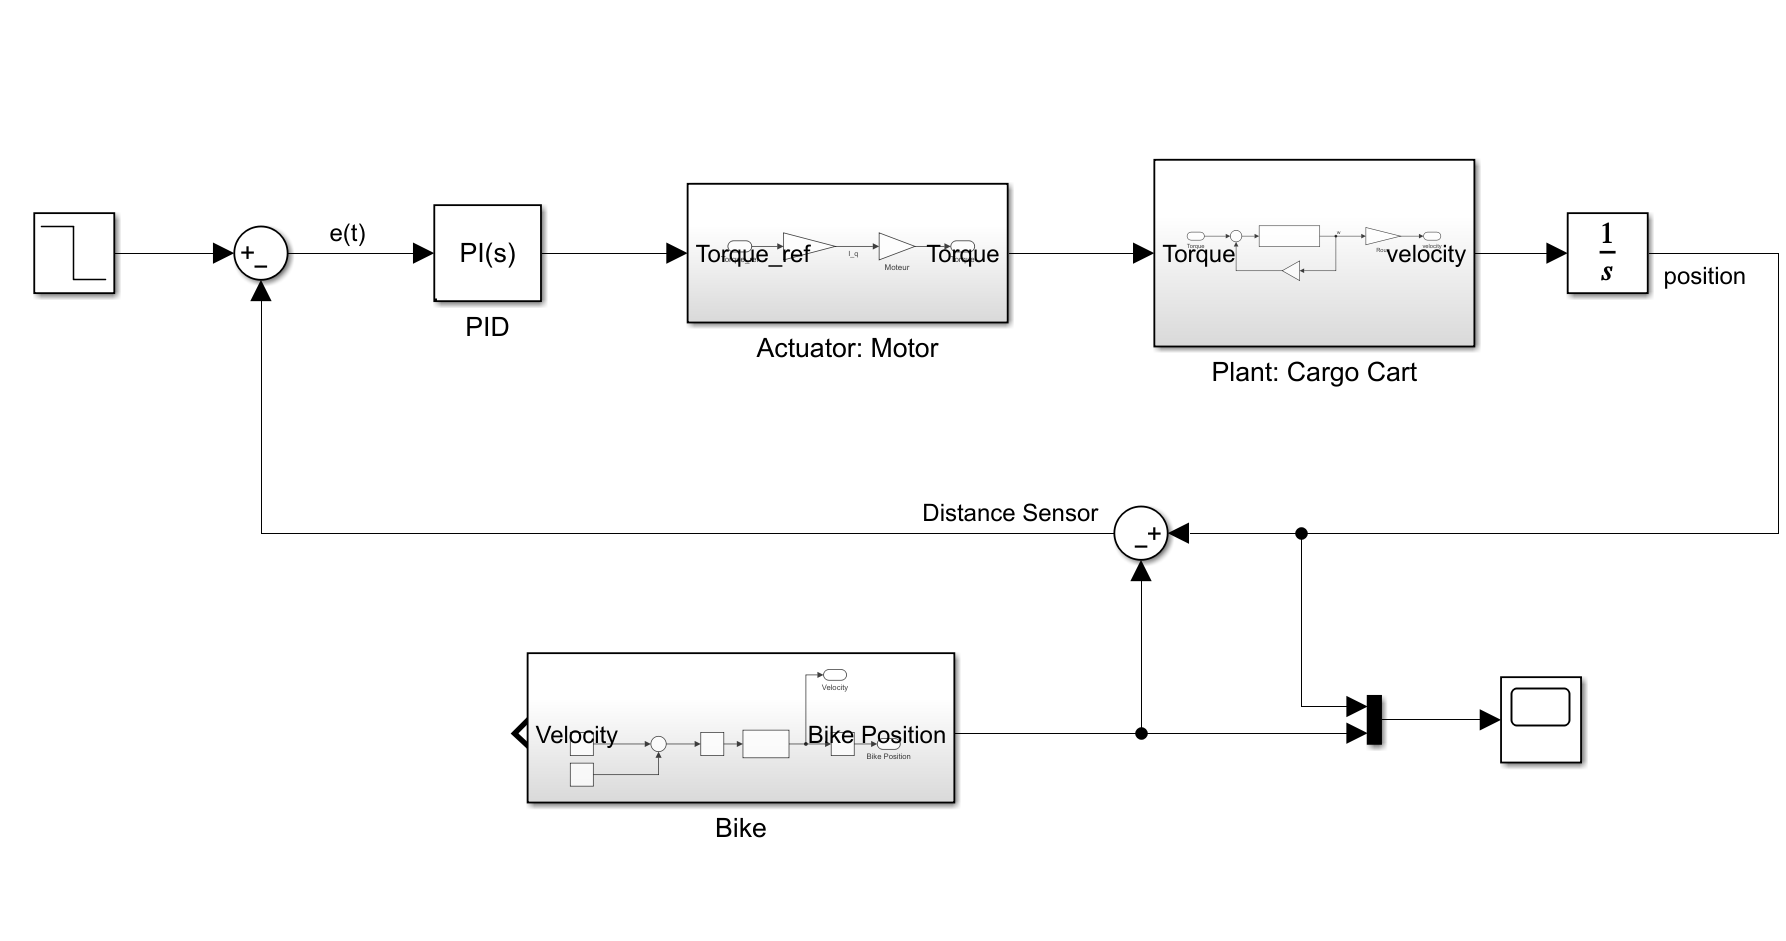
\includegraphics[width=\linewidth]{./Figures/sys_dyn_matlab.png} 
    \caption{Closed-loop model of the bicycle-cargo system with PI control.} 
    \label{fig:simulink-closedloop} 

\end{figure} 


\subsection{Control Architecture Exploration}
Beyond the standard PI control structure simulated in the previous sections, this project explores a more sophisticated control law: the Cascaded Loop Architecture. This approach is envisioned as a high-level software enhancement to meet the robustness and safety requirements inherent to electric cargo mobility. This means that our control law includes two feedback loops that use two different physical parameters. 

The selected cascaded structure is a well-established industry standard, particularly in high-performance motion control and robotics. Similar architectures are widely employed in Automated Guided Vehicles (AGVs) and platooning systems, where a “follower” unit must synchronize its dynamics with a “leader” unit through precise feedback loops.

The proposed approach decomposes the complex task of “cart following” into manageable sub-tasks by nesting control loops: 
\begin{itemize}
    \item Outer loop: Position control layer.
    Using a linear encoder or distance sensor mounted on the trailer’s hitch, the system measures the relative displacement (error) between the bicycle and the cargo cart. This error is processed by a Proportional (P) Controller. The primary goal of this stage is to translate physical distance into a target velocity setpoint. By saturating the output of this loop, we can prevent the cargo cart from ever exceeding the bicycle’s speed, thereby ensuring it never “pushes” the cyclist. 

    \item Inner loop: Velocity control layer.
    The velocity setpoint generated by the outer loop is fed into this internal layer, the inner loop is responsible for commanding the motor torque directly to compensate for immediate mechanical disturbances. Because this loop operates at a higher frequency, it can reject disturbances such as sudden changes in rolling resistance or friction, before they significantly impact the overall position error. 
\end{itemize}

\begin{figure}[!h]

    \centering 
    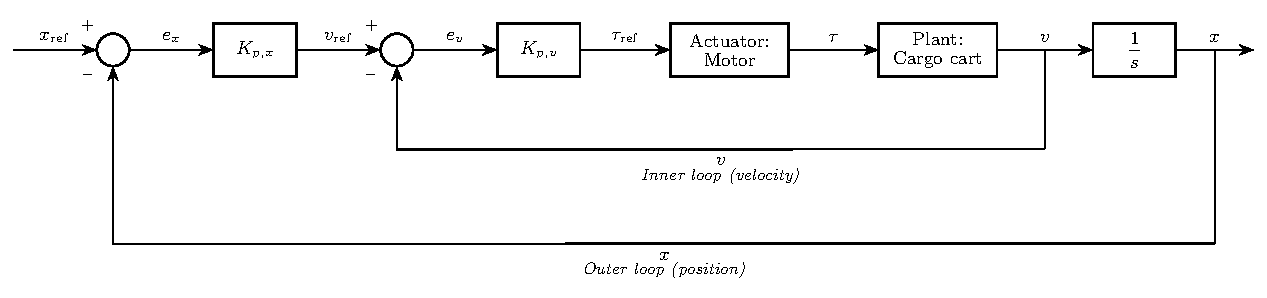
\includegraphics[width=\linewidth]{./Figures/Schema_Autom_PIR.pdf} 
    \caption{Cascaded control architecture for the bicycle-cargo system.} 
    \label{fig:cascaded-loop} 

\end{figure}

Fig.~\ref{fig:cascaded-loop} illustrates the cascade architecture for the dynamics of the cargo cart. In this scheme, $x_{\text{ref}}$ denotes the desired position of the bicycle, whereas $x$ represents the measured position of the cargo cart.

An outer Proportional Controller $K_{p,x}$ converts the position error $e_x = x_{\text{ref}} - x$ into a velocity reference $v_{\text{ref}}$, which serves as the set-point for the inner loop.
The inner Proportional Controller $K_{p,v}$ then transforms the velocity error $e_v = v_{\text{ref}} - v$ into a torque reference $\tau_{\text{ref}}$.
This command is processed by the motor/actuator block, which delivers the actual torque $\tau$.
The model of the plant maps this torque to velocity $v$, and the integrator $1/s$ reconstructs the position $x$.

The adoption of a cascaded loop architecture offers decisive advantages but comes with disadvantages. This precision introduces increased complexity: the multiplication of tuning parameters and the requirement for high-resolution feedback sensors, such as encoders, raise hardware costs and must come with high-performance software. These technical constraints represent a significant challenge and may raise other issues.




